%%%mark = star, diamond, square, otimes
%\documentclass{article}
%\usepackage{pgfplots}
%\usepackage[justification=centering]{caption}
%\pgfplotsset{compat=newest}
%\begin{document}
\begin{figure}
\centering

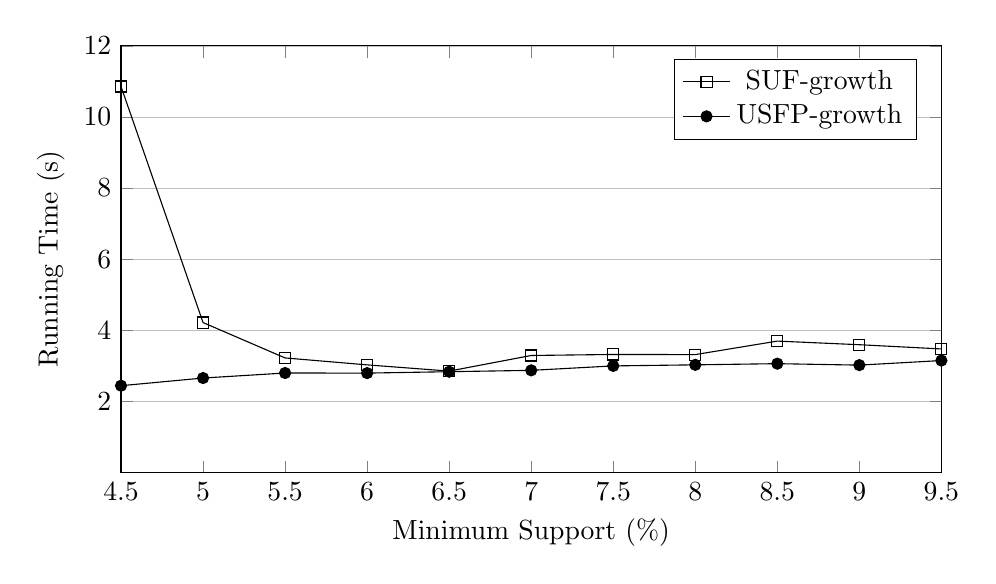
\begin{tikzpicture}
\begin{axis}[
 width=12cm,
   height=7cm,
    xlabel={Minimum Support (\%) },
    ylabel={Running Time (s)},
    xmin=4.5, xmax=9.5,
    ymin=0, ymax=12,
    xtick={4.5,5,5.5,6,6.5,7,7.5,8,8.5,9,9.5},
    ytick={2,4,6,8,10,12},
    legend pos=north east,
    ymajorgrids=true,
    grid style={line width=.2pt,draw=gray!50},
]
 
\addplot[
    solid, every mark/.append style={solid, fill=gray}, mark=square
    ]
    coordinates {
			(4.5,10.856)
			(5  ,4.216 )
			(5.5,3.221 )
			(6  ,3.026 )
			(6.5,2.851 )
			(7  ,3.29  )
			(7.5,3.319 )
			(8  ,3.315 )
			(8.5,3.695 )
			(9  ,3.593 )
			(9.5,3.474 )

};
    \addlegendentry{SUF-growth}
\addplot[
    solid, every mark/.append style={solid, fill=black}, mark=*
    ]
    coordinates {
			(4.5,2.44  )
			(5  ,2.656 )
			(5.5,2.797 )
			(6  ,2.795 )
			(6.5,2.834 )
			(7  ,2.872 )
			(7.5,2.997 )
			(8  ,3.027 )
			(8.5,3.06  )
			(9  ,3.019 )
			(9.5,3.148 )

};
    \addlegendentry{USFP-growth}
 
\end{axis}
\end{tikzpicture}
\caption{Total Tree Mining vs Minimum Suppport (\%) (Window Size = 5, Frame Size = 7000) for T40I10D100K database}
\label{result:t10_mining_total}
\end{figure}
%\end{document}